\documentclass{article}
\usepackage{pythontex}
\usepackage{tabularx}
\usepackage{graphicx}

\title{Using machine learning to predict typing speed}

\newcommand{\code}[1]{\texttt{#1}}

\newenvironment{zeroindent}
  {\par\setlength{\parindent}{0pt}}
  {\par}

\graphicspath{{assets/}}

\begin{document}
\maketitle

\section{Background Information}

One of my hobbies is competitive typing, where I compete with my friends to type a text as quickly as possible. I often use a website called TypeRacer, where your goal is to drive a racecar to the finish line, and the position of your racecar is determined by how many words you've typed correctly in the quote:

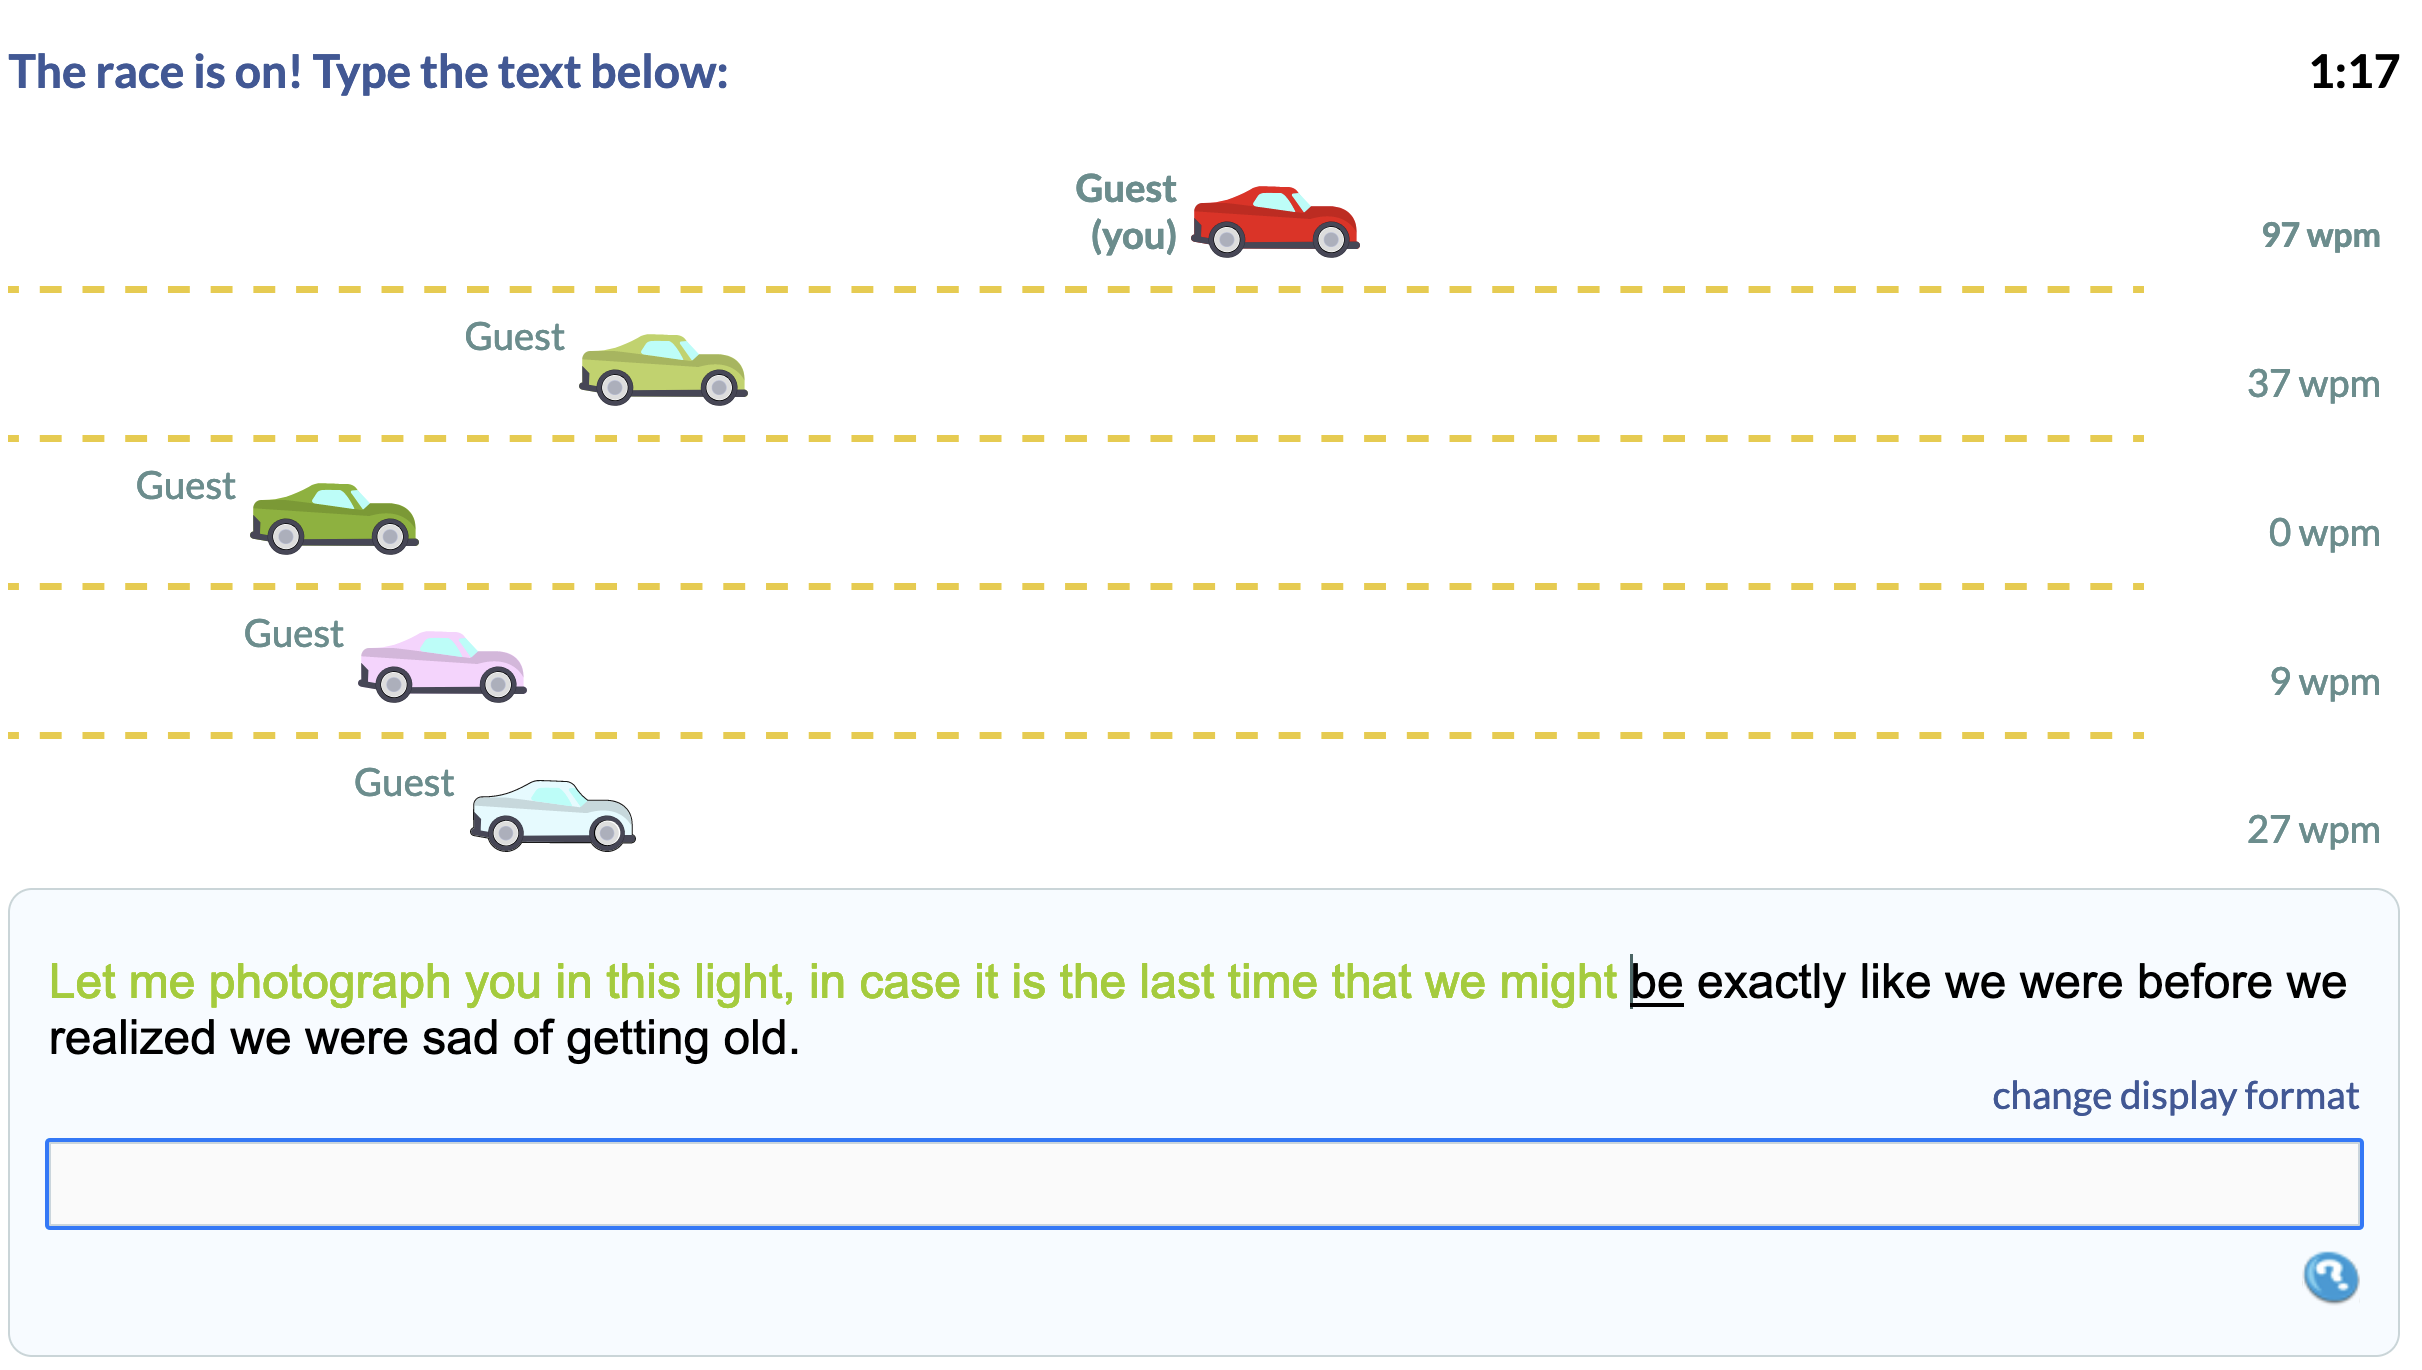
\includegraphics{typeracer.png}

Your score is a measurement of your average typing speed at the end of the race. Typing speed is measured in the units "words per minute" ("wpm" for short), and each word is defined as five characters. Thus, in Figure 1, the

The average typing speed

Touch typing is one of my most useful skills, but it isn't  . I love competing against my friends on TypeRacer, a game where you have to type a certain text faster than o. However, not all texts are created equal.$


Machine learning algorithms is For the scope of this investigation, machine learning is

However, not all texts are created equal. Some texts are harder to type than others, whether it's from having longer, more complex words, frequent capital letters, numbers, etc.

Predicting the difficulty of a text is useful. For example, the typing site that I practice on, TypeRacer, will display different sets of texts depending . For example, these are two quotes that can appear in a TypeRacer race:

\textbf{Quote 1}: Supercalifragilisticexpialidocious is Vielle's favorite word to type on TypeRacer.
\textbf{Quote 2}: For someone who was never meant for this world, I must confess I'm suddenly having a hard time leaving it.

Even though Quote 1 is shorter than Quote 2, the difficult word at the start of Quote 1 makes it significantly more difficult to type.

Currently, the way TypeRacer classifies the difficulty of a newly added quote is through . Each player has an average typing speed that is calculated based on their best scores for each quote, and if the

\section{Data}


Machine learning needs data in order to make predictions.

Since TypeRacer's API doesn't provide data that's sufficiently

\section{Features}

% Script to find average word length of sentences
% \begin{noindent}
\begin{pycode}
import numpy as np

first_sentence = "Someverylongandhardtotypeword and a lot of tiny and short words that are more easy to type."
second_sentence = "Generally, this sentence contains longer and more complex words, but is overall easier to type."

def get_avg_word_length(sentence: str):
	return np.mean([len(word) for word in sentence.split(' ')])

def get_avg_word_length_formatted(sentence: str):
	return "{:.2f}".format(get_avg_word_length(sentence))
\end{pycode}
% \end{noindent}

In a quote, there are often certain parts of the quote that are harder than others. Thus, features that take into account averages like the average word length might not accurately reflect a quote. This problem is demonstrated by the following example:

\medskip

\begin{zeroindent}
	\textbf{Quote 1:} \py{first_sentence}
	\newline
	Average word length: \py{get_avg_word_length_formatted(first_sentence)} words

	\smallskip

	\textbf{Quote 2:} \py{second_sentence}
	\newline
	Average word length: \py{get_avg_word_length_formatted(second_sentence)} words
\end{zeroindent}

\medskip

In the above example, even though Quote 1, has a long word that on its own would be much harder to type, the average word length of the quote overall is.

One possible solution would be analyze each word individually, independent of the others. Then, to predict an overall score, we would sum up the individual speed of each word. However, this approach doesn't account for cases where the words before and after influence the speed at which the word is typed. Consider the following example

\medskip

\begin{zeroindent}
	\textbf{Quote 1:} he HAS a keyboard
	\textbf{Quote 2:} he has a keyboard
\end{zeroindent}

In the first quote, to type \code{HAS}, I need to use my left pinky finger to hold down the shift key while I press the \code{;} key on using my right hand. Then, to type the letter \code{a}, I need to lift up my pinky finger and move it to the /

% \begin{noindent}
\begin{pycode}
row_number = 0

quote_1_wpm = [98, 101, 94, 122, 86]
quote_1_avg = np.mean(quote_1_wpm)

quote_2_wpm = [119, 143, 120, 140, 115]
quote_2_avg = np.mean(quote_2_wpm)

def get_table_1_row(index: int):
	global row_number
	row_number += 1
	return f"\\\\\\hline \n {row_number} & {quote_1_wpm[index]} & {quote_2_wpm[index]}"
\end{pycode}
% \end{noindent}

\begin{tabularx}{\textwidth}{|X|X|X|}
	\hline

	Trial \# & Quote 1 WPM      & Quote 2 WPM

	\py{get_table_1_row(0)}
	\py{get_table_1_row(1)}
	\py{get_table_1_row(2)}
	\py{get_table_1_row(3)}
	\py{get_table_1_row(4)}

	\\\hline
	Average  & \py{quote_1_avg} & \py{quote_2_avg}
	\\\hline
\end{tabularx}

Thus, analyzing the WPM of typing individual words isn't enough.

Instead, we can combine the two above approaches and analyze pairs of words instead, as the speed of a word usually depends on the word before it, since that's usually the word that determines the final locations of finger placements before typing the next word. For example, the following quote:

The quick brown fox jumps

Would be broken down into the following word pairs:

The quick
quick brown
brown fox
fox jumps

Then, using the logs from the race data, we then calculate the wpm of typing each of these word pairs. A dummy result might be:

The quick - 168 wpm
quick brown - 163 wpm
brown fox - 164 wpm
fox jumps - 182 wpm

This process is repeated for every quote and the results are saved. Then, we identify features in each word pair and feed the data into our machine learning algorithm such that it would be able to predict the speed of typing a certain word pair.

To find the average, you first assign the first value to a wpm that's know (i.e. you know how fast typing the individual word would be. This would be another machine learning algorithm of its own: predicting how fast you would type a word if it was the first word of a sentence. I have to use all my quotes but it might not be the most complete data set.).

% \begin{noindent}
\begin{pycode}
features = """
	- How many double letters the word has (double letters are slower to type)
	- How many characters the word has
	- Can't measure every letter combination because there's not enough data (e.g. if I wanted to predict how fast I'd type an abbreviation like "nvm", I don't have enough data on words that have the "nv" or "vm" combination).
	-
"""
\end{pycode}
% \end{noindent}

\begin{itemize}
	\item The numbers of words in the quote
	\item The individual word frequencies
	\item
\end{itemize}

For the purpose of this analysis, we won't be taking into account word accuracy. This is because accuracy is fairly random: just because I type a word wrong in one race doesn't mean that I usually type that word wrong, and just because I've never typed a word wrong doesn't mean I've mastered it. To eliminate this noise, we'll be disregarding mistyped words from the dataset.

\end{document}